\chapter{Implementation} \label{implementation_chapter}
\todo{Legg inn kilde for Left Handed, Z Up coordinate system}
This chapter will look closer into the ideas, code and structure behind various parts of the application. all shown code is written by the project group members. One important aspect of Unreal Engine to remember is that the order of axes might be different than other industry standards, as Unreal Engine uses a Left Handed, Z Up coordinate system. (source) In this three-dimensional space, the \textbf{X}-axis points forwards, the \textbf{Y}-axis points to the right, and the \textbf{Z}-axis points upwards.

\todo{Skriv om blueprints, og pipelinen om prototyping i blueprint til cpp}

\section{Game flow} \label{game_flow}

The flow of the game is mostly handled within \verb|EditorHUD.cpp|. The way Unreal handles level switching is by opening levels based on case sensitive \textit{FName} variables. Level changes happens when a user wants to start a scenario from the main menu, and change back to main menu. To decide if the application should open in editor or simulator mode there is a button in the main menu that allows you to change the mode of the main menu. The implementation of this is fairly easy and is displayed below. All scenarios has a menu mode variable that gets updated when the button gets pressed. This, together with a change in the application layout, is the logic behind the applications ability to both play and edit a level.

\begin{lstlisting}[
    caption={Changing menu mode},
    label={lst:cppdoc},
    language=C++]
void AEditorHUD::ChangeMenuMode()
{
	bMenuMode = !bMenuMode;

	// Changing the options for the Menu scenario
	for (int i = 0; i < ScenarioWidgets.Num(); i++)
	{
		ScenarioWidgets[i]->SetMenuMode(bMenuMode);
	}
	// Changes layout for the menu
	MainMenuWidget->ChangeLayout(bMenuMode);
}
\end{lstlisting}

When a game is opened, the game mode used is either decided by the default blueprint chosen for the level in the editor or it could be set to a gamemode in the options string. Unreal Engine does not yet have a visually appealing approach for handling gamemode changes during runtime, and this statement is supported by the community \cite{ue4_change_gamemode}. The negative aspect of this is that creating the functionality for this may in some cases look a bit messy as shown in the code listing \ref{lst:gamemode} .

\begin{lstlisting}[
    caption={Changing game mode at runtime. The code is not the full implementation, but a modified version to show the changing of game modes at runtime.},
    label=lst:gamemode,
    language=C++]
    FString GameMode;
	GameMode = "?Game=/Game/Blueprints/UI/CDerivedEditor/BP_EditorGameMode.BP_EditorGameMode_C";

	UGameplayStatics::OpenLevel(GetWorld(), MapNameReference, true, GameMode);
}
\end{lstlisting}

Another important aspect of the game flow is how the levels is accessible for the users and for further development. When a new level has been created by a developer, a developer can easily add the level to the main menu through a structure located in the \textit{EditorHUD} blueprint. This implementation works because the blueprint is derived from the \verb|EditorHUD.cpp| file and using the macros \textit{UENUM}, \textit{USTRUCT} or \textit{UPROPERTY} as shown in code listing \ref{lst:uproperty} exposes the variable to the editor and adds it to Unreal Engines memory system \cite{uproperty_macro_explanation}. 

\begin{figure}[H]
\centering
  \begin{minipage}{.48\textwidth}
  \begin{lstlisting}[
    caption={UPROPERTY macro.},
    label={lst:uproperty},
    language=C++]
    USTRUCT(BlueprintType)
struct FMMObjectStruct
{
    GENERATED_BODY();

    UPROPERTY(...)
    ECategoryMM Category = ECategoryMM::ATC;
    UPROPERTY(...)	
    FString Name;
	UPROPERTY(...)
	FString Description;
	UPROPERTY(...)
	FName MapName;
};
UPROPERTY(...)
TArray<FMMObjectStruct> MMObjects; ///< All objects
}
\end{lstlisting}
  \label{fig:test2}
\end{minipage}
\begin{minipage}{.48\textwidth}
  \centering
    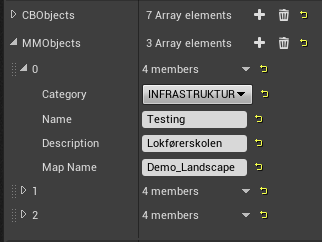
\includegraphics[width=0.90\linewidth]{figures/EditorHUD_MMObjects.PNG}
  \captionof{figure}{The module hierarchy for simulating mode}
  \label{editorMMobj}
  \end{minipage}
\end{figure}

\section{Spline Tool}

One of the first goals specified by the client was to move the train along a straight path. Seeing as a later goal was to also implement curvature, we decided that it would be beneficial to begin work on curved train movement right away, as this would likely save us some time. In the existing simulator, the railway is procedurally generated from a list of points forming a \textit{spline}. A spline can be defined as a mathematical function to interpolate and form a smooth curve between multiple points. Each point is made up of a location vector and a tangent vector for specifying the curvature of the spline at the given position. We also looked into \textit{Bézier curves}, a similar alternative to splines, but Unreal Engine's built-in spline component made it an obvious choice. \newline

\begin{figure}[h]
    \centerline{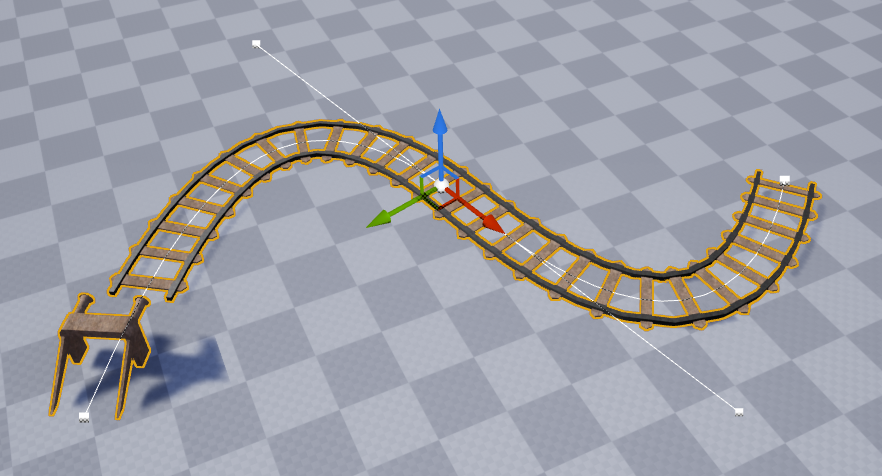
\includegraphics[width=0.9\textwidth]{figures/Spline1.png}}
    \caption{A selected spline deforming a railway mesh along itself. The white squares indicate the spline points, and the white lines indicate the tangent of the selected spline point.}
    \label{SplineFigure}
\end{figure} 


We created \verb|SplineActor.cpp|, a class for handling all functionality related to the railway. This class contains a \textit{USplineComponent}, a powerful component with functions for placing and deforming a mesh along a spline. In this context, a mesh can be described as a 3D-model. The way this initially works is by looping over all points in the spline, placing a sub-mesh that is stretched between points $P_n$ and $P_{n+1}$, and bending the meshes by the curvature of the tangents between $T_n$ and $T_{n+1}$. The spline points were defined by the user in the editor, and could be placed freely. The results looked promising, but a major flaw of this method occurs when any distances between each set of spline points aren't uniform. The meshes would stretch differently along the spline, making the railway look rather odd. A good analogy is imagining a skyscraper with a single, horizontally stretched window instead of separate windows on each floor. The solution to this was to split the spline into segments of equal length to that of the mesh/model itself, and add a new sub-mesh at each segment. Essentially cutting up the railway into pieces and replacing the existing spline points. The mesh used in figure \ref{SplineFigure} is a small slice of a railway created with primitive shapes in \textit{Asset Forge}, a third party software.\footnote{Asset Forge, \url{https://assetforge.io/}} \\

% CODE


% SKAL FJERNE MASSE AV KODEN DONT WORRY "IM WORRIED!!! - HENRIK"

\begin{lstlisting}[
    caption={Initialization of spline points},
    label=lst:cppdoc,
    language=C++]

// Get the size vector of the mesh
const FVector MeshSize = Mesh->GetBoundingBox().GetSize();
	
// Get the length of the bounding box of the mesh along the forward axis
const float MeshLength = MeshSize.X;

...

const float SplineLength = SplineComponent->GetSplineLength();

// Set number of spline points to number of meshes fitting inside spline length
const int SplinePoints = FMath::CeilToInt(SplineLength / MeshLength);

for (int PointCount = 0; PointCount < SplinePoints; PointCount++)
{
	// Generate a spline mesh component for each point in the spline
	USplineMeshComponent* SplineMesh = 
	NewObject<USplineMeshComponent>(
	    this, USplineMeshComponent::StaticClass()
	);

	...
	
	// Get the location and tangents for the mesh at the 
	// current distance along the spline
	
	const float StartDistance = MeshLength * PointCount;
	
	FVector StartPoint = GetLocationAtDistanceAlongSpline(
	    StartDistance, ESplineCoordinateSpace::Local
    );
	    
	FVector StartTangent = GetDirectionAtDistanceAlongSpline(
	    StartDistance, ESplineCoordinateSpace::World
    );
    
	// Get the location and tangents for the end of the 
	// mesh at the current distance along the spline

	const float EndDistance = MeshLength * (PointCount + 1);
	
	FVector EndPoint = GetLocationAtDistanceAlongSpline(
	    EndDistance, ESplineCoordinateSpace::Local
	);
	
	FVector EndTangent = GetDirectionAtDistanceAlongSpline(
	    EndDistance, ESplineCoordinateSpace::World
	);
	
	...
	
	// Set the mesh location and curvature in spline
	SplineMesh->SetStartAndEnd(
	    StartPoint, 
	    StartTangent, 
	    EndPoint, 
	    EndTangent
    );
}
\end{lstlisting}


Opting for a custom spline class instead of Unreal Engine's own solution let us create a railway from a spline. We added specific elements such as \textit{buffer stops}, the metal bars at the end of a railway to stop trains, as seen in figure \ref{SplineFigure}. We added an optional parameter to the \verb|SplineActor.cpp|, where the user can input a separate mesh to be displayed as the first and/or the last sub-mesh of the spline. However, if this field is left empty, the sub-mesh will default to the given railway mesh. We also implemented a boolean flag which sets off if the spline extends a desired angle or curvature limit, to ensure the train looking natural when traversing the railway. \newline

\begin{figure}[h]
    \centerline{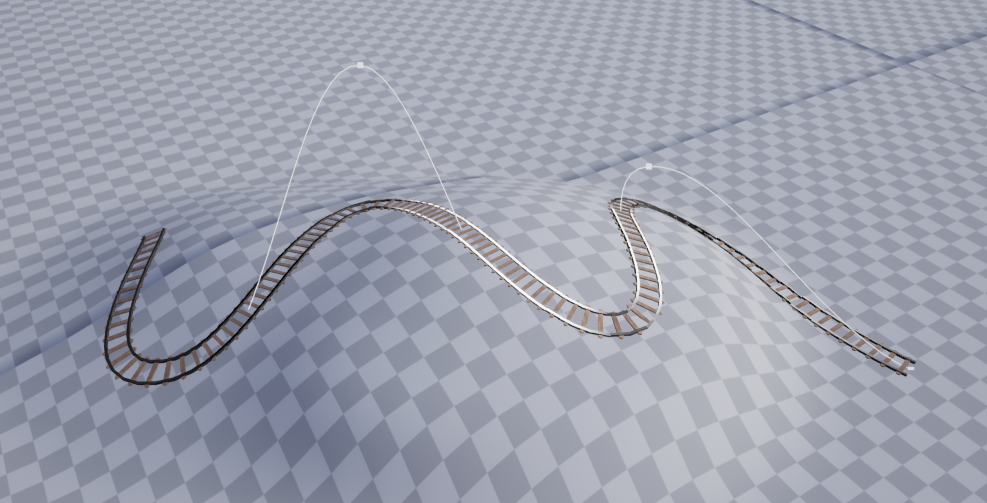
\includegraphics[width=0.9\textwidth]{figures/Spline2.png}}
    \caption{A railway conforming to the terrain height}
\end{figure} 

One of the challenges with the tool occurred when manually placing the spline points. The railway curved naturally in the horizontal plane, but if the terrain had any difference in height, the railway would simply disappear under ground or hover above ground. To solve this, we perform a line cast in each spline point's X- and Y-coordinates, from the top to the bottom of the level. This is a way to see if we hit any terrain along the line cast. If there is a hit, the Z-coordinate of the relevant spline point is simply set to the height value of the terrain hit. This gets more computationally expensive the longer a spline is, but is only run once when a spline undergoes change, so any noticeable effects are minuscule. 
% kjør oppdatering av spline i en annen thread? da slipper editoren å lagge så mye når man endrer på ting. fant en plugin som bruker spline greier i en annen thread, men koster penger. Skal gå ann å lage en ny thread, gjøre computations der og sende det tilbake i game thread. - EH


\section{Signal controller}

The \textit{CentralSignalController} class is responsible for signal and status communication between the signals and trains. The controller receives signal and status updates from either \textit{TrainSignalTriggerBox} or \textit{TrainStatusTriggerBox}, which are placed along the railway and are used to send signal or status updates depending on configured conditions. 

When the level is loaded and the game begins, the \textit{CentralSignalController} searches for all actors inheriting from the \textit{BasicSignal} class. Valid actors are then sorted into lists based on which type they are, such as \textit{MainSignal} or \textit{ForwardSignal}. These different lists are then used later to send signal updates. 

\begin{lstlisting}[
    caption={Finds and stores all signals based on class},
    label={lst:signal_find_signals},
    language=C++]
void ACentralSignalController::FindAllSignals()
{
	// Finds all actors of signal classes
	UGameplayStatics::GetAllActorsOfClass(GetWorld(), DwarfSignalBP, DwarfSignalActors);
	UGameplayStatics::GetAllActorsOfClass(GetWorld(), MainSignalBP, MainSignalActors);
	UGameplayStatics::GetAllActorsOfClass(GetWorld(), ForwardSignalBP, ForwardSignalActors);

	int32 i = 1;

	// Loops through all actors
	for (AActor* DwarfSignalActor : DwarfSignalActors)
	{
		ABasicSignal* DwarfSignal = Cast<ABasicSignal>(DwarfSignalActor);
		if (DwarfSignal)
		{
			FString TagName = FString::Printf(TEXT("Dwarf_%i"), i++);
			
			DwarfSignal->Tags.Add(FName(TagName));

			AllSignalActors.Add(DwarfSignalActor);
		}
	}
	...
}
\end{lstlisting}

When the controller receives a signal update, an ID, new signal state and signal type must be specified. The controller then searches through the specified signal list to match the IDs, and when this happens the new signal state is sent. The controller continues searching the list, if more than one signal shares the same ID. Given that the length of the list of signals is quite short, the time spent searching the list even when the first match is found is insignificant. % measure this? or at least prove the time spent will have a small to none effect on fps

\begin{lstlisting}[
    caption={Updates signals based on ID and type},
    label={lst:signal_updates},
    language=C++]
void ACentralSignalController::SendUpdatedSignal(FName SignalID, ESignalType SignalType, ESignalStatus Status)
{
	TArray<AActor*> Actors;

	// Selects relevant actors to search based on signal type
	switch (SignalType)
	{
	case ESignalType::Main:
		Actors = MainSignalActors;
		break;
	case ESignalType::Forward:
		Actors = ForwardSignalActors;
		break;
	case ESignalType::Dwarf:
		Actors = DwarfSignalActors;
		break;
	default:
		checkNoEntry();
		break;
	}

	// Loops through all signals
	for (AActor* SignalActor : Actors)
	{
		ABasicSignal* Signal = Cast<ABasicSignal>(SignalActor);
		if (Signal && (Signal->ID == SignalID))
		{
			// If the signal matches the incoming id, update the status
			Signal->UpdateSignalStatus(Status);
		}
	}
}
\end{lstlisting}

As the Central Signal Controller is an actor, it needs to be placed in every level which is going to use signals. One alternative would be to create a subsystem with the same functionality. This would allow the controller to work in any level without needing to place an actor, as well as having a more predictable and stable lifecycle. 

\section{Signals}

The class \textit{ABasicSignal} is used for the three different types of signals. The three signal types share the same functionality, with the only difference being the models used and number of lights on each model, as well as which colors are used and how the signal reacts to signal status updates. 

Each signal type is stored as a blueprint which stores the model used, as well as signal-type specific information such as what colors are used and how the signal reacts to signal status updates. This way only one \cpp code file is used for all signals, which makes it easier to implement new features or fix bugs, in addition to improving maintainability. 

\begin{figure}[h]
    \centerline{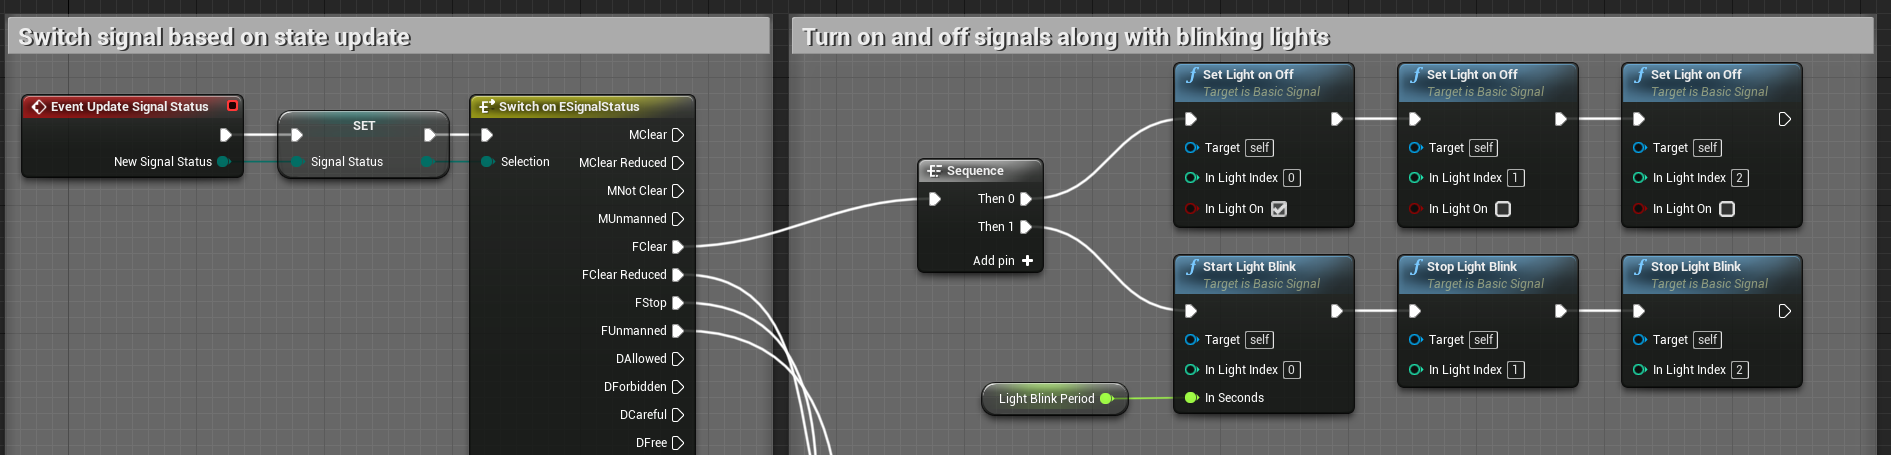
\includegraphics[width=1\textwidth]{figures/Signal_switch.png}}
    \caption{Blueprint showing how a signal switches status}
\end{figure} 

Because the different signals use different models, hard-coding the positions of the signal lights is not an option. Instead sockets are placed on the models in the Unreal Editor, which are used to dynamically place signal lights at runtime. When the game starts playing spheres are created and placed according to the sockets on the model. A standard naming convention is used for sockets and components. The socket names need to match the socket names on the static mesh model, in order for the positioning to be correct. 

When components are created during runtime it is important to manually register the component, otherwise it will immediately be garbage collected and disappear. \todo{this was an interesting bug/issue to learn about, write more about it?}

\begin{lstlisting}[
    caption={Creates dynamic instanced materials for each signal light},
    label={lst:signal_lights},
    language=C++]
void ABasicSignal::SetupLight()
{
	RemoveLights();

	// Create all lights in a loop
	for (int32 i = 0; i < NumLights; i++)
	{
		FString SocketName = FString::Printf(TEXT("Socket_%i"), i + 1);
		FString LightMeshName = FString::Printf(TEXT("LightMesh_%i"), i + 1);

		UStaticMeshComponent* LightMesh = NewObject<UStaticMeshComponent>(this, FName(LightMeshName));

		// Creates a new light struct
		FSignalLight NewLight(LightMesh);

		NewLight.LightMesh->SetStaticMesh(BaseLightMesh);

		NewLight.LightMesh->SetupAttachment(VisualComponent, FName(SocketName));

		// Creates the instanced dynamic light material
		NewLight.DynMaterial = UMaterialInstanceDynamic::Create(BaseLightMaterial, this);

		NewLight.DynMaterial->SetScalarParameterValue("Emissive_Strength", MaxLightLevel);
		NewLight.DynMaterial->SetVectorParameterValue("Emissive_Color", FLinearColor(1.0f, 1.0f, 1.0f));

		NewLight.LightMesh->SetMaterial(0, NewLight.DynMaterial);

		NewLight.LightMesh->RegisterComponent();


		Lights.Add(NewLight);
	}
}
\end{lstlisting}

A new \Gls{instanced dynamic material} is created for each sphere, which uses emissive lighting for the signal lights. The new dynamic instance of the material allows material parameters to be changed during runtime for each different instance, ensuring the lights can change independent of other light signals of the same type. 

\begin{figure}[h]
    \centerline{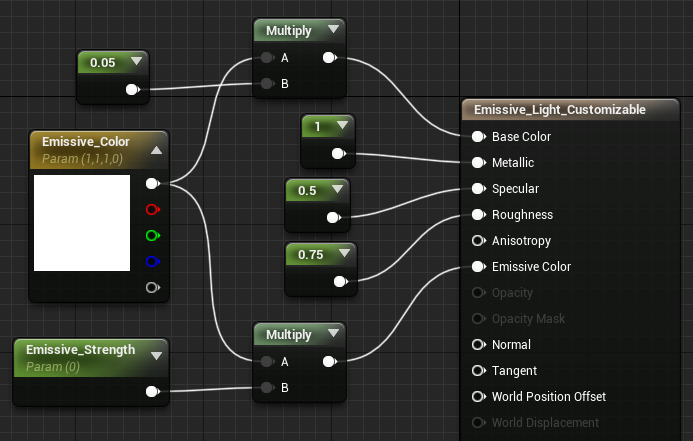
\includegraphics[width=0.9\textwidth]{figures/Emissive_Light_Material.png}}
    \caption{The material used for signal lights}
\end{figure}

The material used for the signal lights is created from scratch in Unreal, using its Material Editor tool. The material has two public parameters which are used to change the color of the material as well as the brightness of the \Gls{emissive light}. The material uses the same color for both the base color and emissive color. The base color has a constant low brightness, which is used for the off state. The emissive color strength is determined by a parameter. All values used range from 0 to 1, with the exception of emissive light strength which can be any value above 0. Higher values results in brighter emissive lights. Currently the entire model using the material lights up as an emissive light source, but a texture could be used to only use parts of the model as an emissive light source.


\section{Login and authentication}

The \textit{ULoginWidget} class contains the functionality used to log in, which uses the \textit{VaRest} plugin to encode, decode, send, and receive web requests. The user data is stored in a struct in \textit{UDesksimGameInstance}, which is a class that is instantiated at the beginning of the application and lives until it is closed, ensuring the user data is available for the entire duration of the application. 

Our application connects with the existing login solution in use at Lokførerskolen. Two endpoints are used, where the first takes a username and password and returns a \acrfull{jwt} on success. The second endpoint takes this \acrfull{jwt} and returns a user object containing various data. This data is then decoded and stored in the gameinstance class, \textit{UDesksimGameInstance}. The application does not verify the \acrfull{jwt} in any way, it just passes it on to the next endpoint. While the \acrfull{jwt} is valid for a long duration, it is not stored in any files, and a new token is requested each time the user logs in. 

% vis kode som decoder og lagrer login info
\begin{lstlisting}[
    caption={Decodes and stores info from userinfo JSON response},
    label={lst:auth_userinfo},
    language=C++]
void ULoginWidget::ReadUserData(UVaRestJsonObject* JsonObj)
{
	UDesksimGameInstance* GameInstance = Cast<UDesksimGameInstance>(GetGameInstance());

	GameInstance->bIsLoggedIn = true;

	// Set Userinfo in gameinstance
	GameInstance->UserInfo.bIsAuthenticated = true;
	
	GameInstance->UserInfo.bIsEnabled = JsonObj->GetBoolField(TEXT("isEnabled"));
	
	GameInstance->UserInfo.id = JsonObj->GetIntegerField(TEXT("id"));
	
	GameInstance->UserInfo.Username = FName(*JsonObj->GetStringField(TEXT("username")));
	
	GameInstance->UserInfo.SubscriptionID = JsonObj->GetIntegerField(TEXT("subscriptionId"));


	// Find info about subscription and user groups
	UVaRestJsonObject* Subscription = JsonObj->GetObjectField(TEXT("subscription"));
	
	TArray<FString> GroupNames = Subscription->GetStringArrayField(TEXT("userGroupNames"));

	// Checks which type the user is
	if (GroupNames.Contains("Administrator"))
	{
		GameInstance->UserInfo.UserType = EUserType::Admin;
	}
	else if (GroupNames.Contains("Ansatte"))
	{
		GameInstance->UserInfo.UserType = EUserType::Teacher;
	}
	else //if (GroupNames.Contains("Student"))
	{
		GameInstance->UserInfo.UserType = EUserType::Student;
	}
}
\end{lstlisting}

The login functionality uses the VaRest plugin to handle common tasks like encoding and decoding \acrshort{json} objects. The plugin was chosen to simplify the use of REST communication.

\section{Editor Mode}
The goal of the editor mode was to give the client a simple tool build worlds and train scenarios. Our task was to implement the ability to place, move and rotate objects such as trains and buildings, and a way to lay a railway across the terrain. We decided to design this tool based on the tools available in Unreal Engine's own editor, as these would accomplish similar tasks. For moving objects around, we created a \gls{gizmo} consisting of one arrow for each axis, and a square for the plane along the X- and Y-axes. Once an object is selected, this gizmo appears at its position, utilizing custom depth rendering, which enables the gizmo to always be visible even when it is covered by another mesh. 

\begin{figure}[h]
\centering
\begin{minipage}{.5\textwidth}
  \centering
  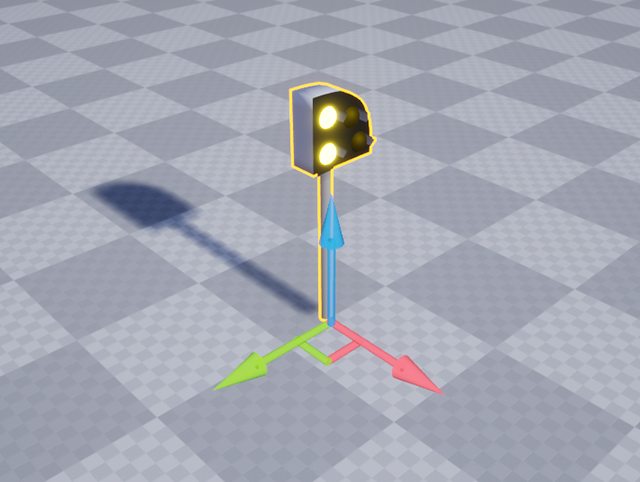
\includegraphics[width=0.95\linewidth]{figures/Gizmo1.png}
  \captionof{figure}{The translation gizmo on a selected signal}
  \label{fig:test1}
\end{minipage}%
\begin{minipage}{.5\textwidth}
  \centering
  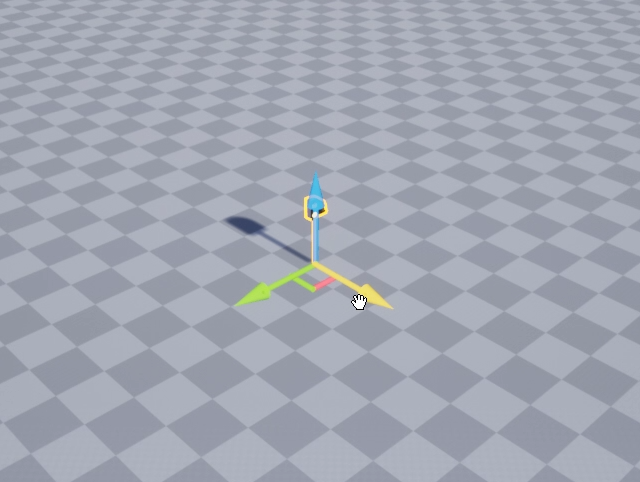
\includegraphics[width=0.95\linewidth]{figures/Gizmo2.png}
  \captionof{figure}{The translation gizmo far away, hovering the X-axis arrow}
  \label{fig:test2}
\end{minipage}
\end{figure}

By hovering the mouse over one of the gizmo's arrows and dragging, the user can move the object in the relevant axis. This is done by casting a line from the camera, in the direction of the cursor's position on the screen, and processing the results on hit. This is done in a separate collision layer for gizmos, such that the line is not obscured by any object. The tool includes two modes, translation and rotation. When switching mode to rotation, the arrow meshes are replaced by a cogwheel in the XY-plane, which rotates the object around the Z axis when dragged. These gizmos are made to be a part of the user interface, and get scaled based on their distance from the camera to keep their size uniform. 

When grabbing a gizmo arrow to move an object, the position of the cursor is saved as a variable in the first frame of holding down the mouse button. This position is used to get the offset between the gizmos center position (also the object anchor position), and the cursor. While dragging the gizmo arrow, the objects position is set to the location of the cursor minus the offset, resulting in the object moving in parallel with the cursor. This behaviour works fine in theory, but during testing, we found a lack of user friendliness due to the cursor being required to overlap the gizmo during dragging. To combat this, we added secondary meshes to each arrow that would inflate the area of interaction. These meshes were given an invisible material, so the user could not see them, but were able to interact with them.

\begin{figure}[h]
\centering
\begin{minipage}{.5\textwidth}
  \centering
  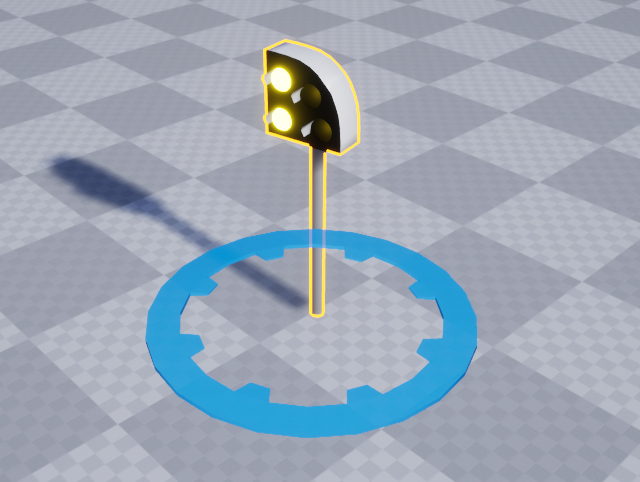
\includegraphics[width=0.95\linewidth]{figures/Gizmo3.png}
  \captionof{figure}{The rotation gizmo in the XY-plane}
  \label{fig:test1}
\end{minipage}%
\begin{minipage}{.5\textwidth}
  \centering
  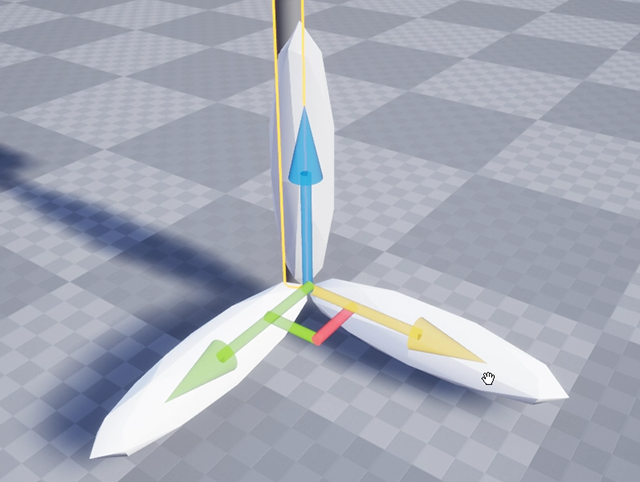
\includegraphics[width=0.95\linewidth]{figures/Gizmo4.png}
  \captionof{figure}{Additional meshes around the arrows}
  \label{fig:test2}
\end{minipage}
\end{figure}

\todo{Forklar litt rundt figurene i teksten}

During user testing with the client, it was made clear that this interaction was still hard, as the cursor would, more often that not, exit the area of these meshes. This was towards the very end of the development, and there was not enough time to iterate on this implementation, as it would quickly grow complicated. But due to the curious nature of programmers, we were attracted towards finding a solution to this problem, even if we did not have the time to finish the implementation of these ideas. We came up with several possible solutions that could fix or recreate this system entirely.


One such idea was to spawn large collision planes at the objects position, when the mouse is dragging an arrow. If the user is moving the object, the plane should stretch like a wall along the relevant axis. It should not be visible to the player, but act as a giant safety net, such as the ones seen at golf courts, to capture the depth of the mouse cursor in the relevant axis. This would provide a more intuitive movement system, where the user could drag the object to it's desired position without keeping the cursor over the gizmo at all times. Another idea for a solution would be to take the cursor's two-dimensional position on the screen and rotate the vector based on the angle between the camera and the object. This may also result in clunky movement, as 2D does not always translate well to 3D when forced.

\section{Landscape and texturing}
% Landscape texture - John Ole 


There was originally a planned runtime terrain editing tool for the simulator, but it became obvious that such functionality would take a considerable amount of time and was therefore taken out of the project scope. This will be further discussed in [discussion::editor] 
\todo{Link discussion}

\section{Save Functionality}
The meaning of saving the game can vary from game to game, but the idea behind it is to save information about something persistent. Say you quit and re-open the game, you should be able to resume where you left off. In this project we have implemented an editor mode where the player can edit and change the world/level they are playing. But for the editor mode to serve its purpose we need to be able to save the changes we made to the level so we can open it in play mode after and view the changes. 

Our \textit{SaveLevel} class inherits from Unreal`s \textit{SaveGame} class which is used to preserve information across multiple play sessions. We mainly save the transform of placed or edited objects in the scene, but also general data and identifiable data such as name, class and level name. All the information from the actors saved is stored inside a array in a \verb|.sav| file which is the save file format Unreal Engine 4 uses.

\todo{code caption and label}

\begin{lstlisting}[
    caption={SaveLevel class that holds all data that is saved},
    label={lst:SKRIVHER},
    language=C++]
/**
 * @brief Struct holding all Data needed from an Actor.
 */
USTRUCT()
struct FActorData
{
    ...

public:
    /* Identifier for which Actor this belongs to */
    UPROPERTY()
        FName Name;
	
    /* Class of the Actor */
    UPROPERTY()
        UClass* Class = nullptr;;

    /* For movable Actors, keep location,rotation,scale. */
    UPROPERTY()
        FTransform Transform;

    /* Contains all 'SaveGame' marked variables of the Actor */
    UPROPERTY()
        TArray<uint8> ByteData;
};

/**
 * @brief Handles what data is saved in the .sav files.
 */
UCLASS()
class DESKSIMV2_API USaveLevel : public USaveGame
{
	...

public:
    ...

    UPROPERTY()
        TArray<FActorData> SavedActors;

    ...
};
\end{lstlisting}

A big issue we had was how we would handle what actors got saved, since a level can often contain many actors many of which we do not edit or create in editor mode and it would be unnecessary to save those actors. We explored different options one of which was to create a base actor class which every save able actor inherits. Although this would not work since the save able actors are of different classes. Instead we created an interface the actors can inherit if they are save able, giving every class the ability to be saved regardless of what their base class is.

\begin{lstlisting}[
    caption={Interface for classes that are save able},
    label={lst:SKRIVHER},
    language=C++]
UINTERFACE(MinimalAPI)
class UIsSaveableInterface : public UInterface
{
	GENERATED_BODY()
};

/**
 * 
 */
class DESKSIMV2_API IIsSaveableInterface
{
	GENERATED_BODY()

	// Add interface functions to this class. This is the class that will be inherited to implement this interface.
public:
};
\end{lstlisting}

An example of how a class can be made saveable by inheriting the interface in the class declaration along side their parent class.

\begin{lstlisting}[
    caption={Example of a class that inherits IsSaveableInterface},
    label={lst:SKRIVHER},
    language=C++]
UCLASS()
class DESKSIMV2_API ATrain : public APawn, public IIsSaveableInterface
{
	...
\end{lstlisting}

All the save functionality is handled by the \textit{SaveManager} which has two main functions, \textit{SaveGame} and \textit{LoadGame}. \textit{SaveGame} handles all the functionality related to saving the current game state into a \verb|.sav| file. It checks all actors classes in the level and if it inherits from the \textit{IsSaveableInterface} interface its data is saved. 

\begin{lstlisting}[
    caption={SaveGame function from SaveManager},
    label={lst:SKRIVHER},
    language=C++]
void ASaveManager::SaveGame()
{
	// Get LevelName to find what to name the .sav file
	LevelName = GetWorld()->GetMapName();

	// Create and instance of SaveGame
	USaveLevel* SaveGameInstance = Cast<USaveLevel>(UGameplayStatics::CreateSaveGameObject(USaveLevel::StaticClass()));
	check(SaveGameInstance);
	// Loop through ALL Actors in Scene
	for (TActorIterator<AActor> It(GetWorld()); It; ++It)
	{
		// Checks if the Actor inherits from IsSaveableInterface
		if (It->GetClass()->ImplementsInterface(UIsSaveableInterface::StaticClass())) 
		{
			AActor* Actor = *It;

			FActorData ActorData;
			ActorData.Name = Actor->GetFName();
			ActorData.Transform = Actor->GetActorTransform();
			ActorData.Class = Actor->GetClass();

			// Creates a memorywriter and archive for Actor Data
			FMemoryWriter MemWriter(ActorData.ByteData);
			FObjectAndNameAsStringProxyArchive Ar(MemWriter, true);
				
			// Only Saves Variables with UPROPERTY(SaveGame)
			Ar.ArIsSaveGame = true;
				
			// Serializes Actors UPROPERTIES into binary
			Actor->Serialize(Ar);
				

			SaveGameInstance->SavedActors.Add(ActorData);
		}
	}

	// Start async save process.
	UGameplayStatics::SaveGameToSlot(SaveGameInstance, LevelName, UserIndex);

	...
}
\end{lstlisting}

The \textit{LoadGame} function in \textit{SaveManager} reads and loads data of the \verb|.sav|-file with the matching file name to the name of the loaded level. Then it updates the data of the existing actors with the matching data from the save file based on the actors name. If it doesn't find the actor from the savefile in the level it will create a new actor with the data from the save file.


\begin{lstlisting}[
    caption={LoadGame function from SaveManager},
    label={lst:SKRIVHER},
    language=C++]
void ASaveManager::LoadGame()
{
	// Get LevelName to find what .sav file to load
	if (!GetWorld()) return;
	
	LevelName = GetWorld()->GetMapName();

	// Create and instance of SaveGame
	USaveLevel* SaveGameInstance = Cast<USaveLevel>(UGameplayStatics::CreateSaveGameObject(USaveLevel::StaticClass()));
	check(SaveGameInstance);
	

	// Load Data from Save file
	SaveGameInstance = Cast<USaveLevel>(UGameplayStatics::LoadGameFromSlot(LevelName, UserIndex));
	if (SaveGameInstance)
	{
		// Iterate through all actors in save and point to their corresponding actor in scene
		for (FActorData ActorData : SaveGameInstance->SavedActors)
		{
			AActor* Actor = FindActorByName(ActorData.Name);
			if (Actor)
			{
				// Updates Actor found in scene
			    Actor->SetActorTransform(ActorData.Transform);
			}
			else
			{
				FActorSpawnParameters SpawnParams;
				SpawnParams.Name = ActorData.Name;
				SpawnParams.SpawnCollisionHandlingOverride = ESpawnActorCollisionHandlingMethod::AdjustIfPossibleButAlwaysSpawn;
					
				// Creates a new Actor with data from save
				Actor = GetWorld()->SpawnActor(ActorData.Class, &ActorData.Transform, SpawnParams);
					
				// Creates a memoryreader and FArchive
				FMemoryReader MemReader(ActorData.ByteData);
				FObjectAndNameAsStringProxyArchive Ar(MemReader, true);

				// Only Filters the Variables with UPROPERTY(SaveGame)
				Ar.ArIsSaveGame = true;

				// Converts serialized binary into Actors UPROPERTIES
				Actor->Serialize(Ar);
					
				...
			}
		}
		...
	}
	...
}
\end{lstlisting}

\section{User Interface / Heads-Up Display} \label{HUD_implementation}

The heads up displays or HUDs of the application is in the context of the simulator a term used to describe all user interface elements in the simulator to provide feedback to the user in the viewport. 

The HUD consist of seven different user widgets. User widgets are Unreal Engine's components that allows for placement of UI elements in the viewport for 3D games. This section will explain the development of the logic that displays the user widgets.

In the first iteration of the user widgets they were created as \gls{blueprint}, this meant that all of the widgets with it's logic was created as a collection of nodes. According to the Unreal Engine forum, blueprints run between 10-40 percent slower than \cpp \cite{ue4_blueprint_forums_2016}. This was one of the reasons we felt that it was necessary to convert the code from blueprint to \cpp files. Another fact is that blueprint coding, as a practise, does not allow us as students to display our skills in both programming and documentation to the same degree.

\begin{figure}[H]
    \centerline{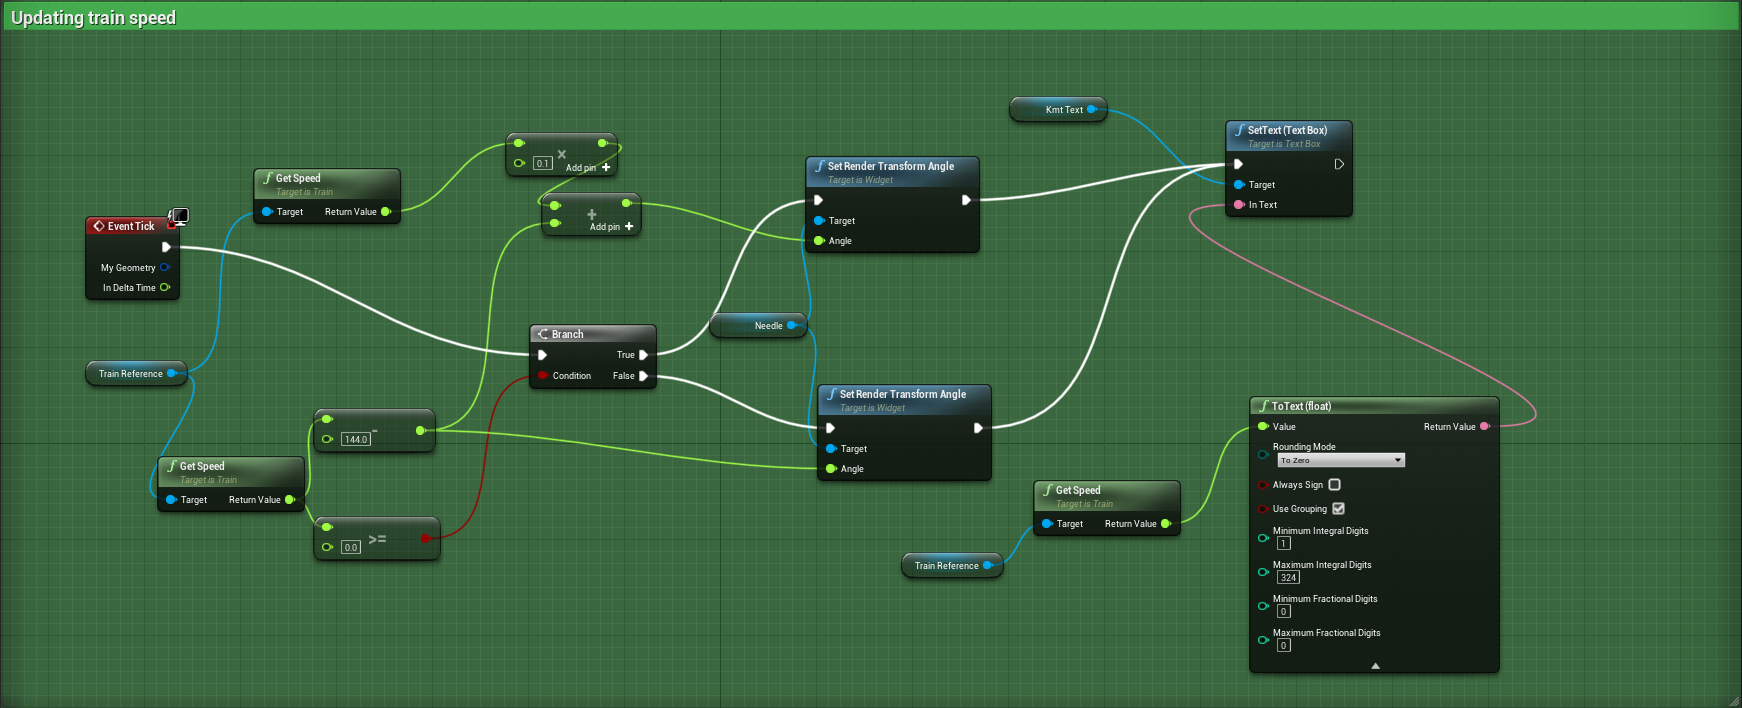
\includegraphics[width=0.9\textwidth]{figures/TrainDMISpeedFunc.PNG}}
    \caption{Update Speed function for the train DMI in blueprint}
    \label{fig:train_dmi}
\end{figure}

Figure \ref{fig:train_dmi} and code listing \ref{lst:updateDMI} contain the same functionality for updating the needle and text of the speedometer displayed to the user. All of the widgets initially created as blueprints got converted to \cpp at some point in the project.

\begin{lstlisting}[
    caption={Update speed function in \cpp},
    label={lst:updateDMI},
    language=C++]
void UTrainDMI::Update(float Speed)
{
	if (Speed >= 0.0)
	{
		float RenderAngleDriving = (Speed * 0.1) + (Speed - 144);

		int Text = FMath::FloorToInt(Speed);
		FString SpeedText = FString::SanitizeFloat(Text, 0);

		UpdateDMI(RenderAngleDriving, FText::FromString(SpeedText));
	}
	else
	{

		int Text = FMath::FloorToInt(Speed);
		FString SpeedText = FString::SanitizeFloat(Text);

		UpdateDMI(Speed - 144, FText::FromString(SpeedText));
	}
}
\end{lstlisting}

The file \verb|EditorHUD.cpp| handles which user widget that is displayed to the user. What the HUD displays is based on what game mode that the game is currently using. The game mode is decided by which part of the application the user is currently in. If the user is in the simulator game mode, the train DMI will be displayed.


\section{Plugins}

The following functionality described in this section is not developed by us but needs to be included as it is used in the simulator.

Unreal Engine did not support the usage of two similar input devices using raw input. We therefore decided to look for the options at hand to solve this issue. The two solutions we found was to purchase and utilize a plug-in created by \textit{Lemontmoon} called \textit{VM Input Manager}\footnotemark[1], or to implement an input mapping system to our own application. We chose to utilize the plug-in and the choice and other options will be described in \todo{Described in discussion}
\footnotetext[1]{\url{https://www.unrealengine.com/marketplace/en-US/product/wm-input-manager}}

The plug-in consists of 18 \cpp classes and 31 blueprints. The benefit this had to our project was that we could just manually map the USB input peripherals during run-time. The plug-in is used only used in the \textit{BP\_GameplayGamemodeBase} blueprint to spawn the necessary widget as a red dot in the top left of the screen. 

The \textit{VaRest} plugin handles common tasks related to performing REST calls. It simplifies the process of working with requests and responses, and provides functions to both simplified and detailed ways to create and send requests. While the plugin is designed to be used in blueprints without any \cpp code, all the functionality is available to be used in \cpp. The same results could be achieved without the use of the \textit{VaRest} plugin, however it would require more work unrelated to the main goal. 